\documentclass{beamer}
\usepackage{graphicx}
\setbeamersize{text margin left=20pt,text margin right=20pt}

\begin{document}
\title{Estimating Search Tree Size with Duplicate Detection}
\subtitle{Levi H.S. Lelis, Roni Stern, Nathan R. Sturtevant (2014)}
\author{Presentation by Sean Dobson}

\frame{\titlepage}

\begin{frame}
  \frametitle{General Problem}
  \begin{itemize}
  \item Predict the run time of a search algorithm (quickly).
  \item Think about the assignment we did:
    \begin{itemize}
    \item Which heuristic should we choose?
    \item How can we tell, prior to running the searches, which will be the fastest?
    \item Any gain from choosing the best search could be outweighed by the extra time taken to predict which search is best.
    \end{itemize}
  \end{itemize}
\end{frame}

\begin{frame}
  \frametitle{Specific Problem}
  \begin{itemize}
  \item Predict the number of nodes expanded by the search.
    \begin{itemize}
    \item Not the only factor that decides search run-time.
    \end{itemize}
  \item Account for search algorithms that use duplicate detection (Graph Search).
    \begin{itemize}
    \item Pruning duplicates can greatly reduce the number of nodes expanded.
    \item But it adds an extra layer of complexity to the problem.
    \item How do we predict the number of nodes pruned by duplicate detection?
    \end{itemize}
  \end{itemize}
  \centering
  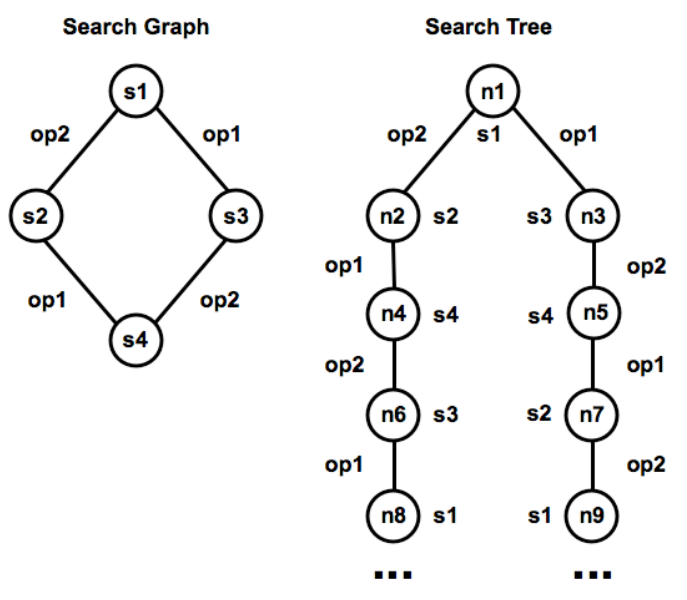
\includegraphics[scale=0.25]{lelis_fig1.png} 
\end{frame}

\begin{frame}
  \frametitle{Claims}
  \begin{itemize}
  \item Stratified Sampling (SS) can be used to predict the number of nodes expanded by Tree Search.
    \begin{itemize}
    \item The algorithm is non-deterministic.
    \item Run it multiple times, and then average (or max) over the outputs.
    \item As the number of 'probes' approaches infinity, the prediction converges to the true value.
    \end{itemize}
  \item Sampling-based Duplicate Detection (SDD) can determine if a node is a duplicate.
    \begin{itemize}
    \item Similar reasoning to above.
    \end{itemize}
  \end{itemize}
\end{frame}

\begin{frame}
  \frametitle{Claims (cont.)}
  \begin{itemize}
  \item Stratified Sampling with Duplicate Detection (SSDD),
    can predict the number of states expanded by Graph Search.
  \item With a little extra work, we can easily account for nodes pruned by A*'s heuristic.
  \item Another variation of the algorithm can be used to predict the state-space radius
  \end{itemize}
\end{frame}

\begin{frame}
  \frametitle{Approach: Type Systems}
  \begin{itemize}
  \item Many-to-one mapping from states to types (a partition of the state space).
  \item An example type system for the 8 Tile Puzzle, based on the position of the blank:
    $$
    \begin{bmatrix}
      c & s & c \\
      s & m & s \\
      c & s & c
    \end{bmatrix},
    \text{ }
    t \left(
    \begin{bmatrix}
      1 & 2 & 3 \\
      4 & 5 & 6 \\
      7 & 8 & B
    \end{bmatrix}
    \right) = c
    $$
  \item
    Note that expanding a type \(c\) will always generate two type \(s\) nodes,
    expanding an \(s\) will generate two \(c\) + one \(m\),
    and expanding an \(m\) will generate four \(s\).
  \end{itemize}
\end{frame}

\begin{frame}
  \frametitle{Example: Predicting 8-Puzzle Search Tree Size}
  \begin{itemize}
  \item \(w_{c,d+1} = 2w_{s,d}\)\\
    \(w_{s,d+1} = 2w_{c,d} + 4w_{m,d}\) \\
    \(w_{m,d+1} = w_{s,d}\)
    \end{itemize}
  \begin{tabular}{r | l | l | l | l | l | l}
     & 0 & 1 & 2 & 3 & 4 & \ldots \\
    \hline
    \(c\) & 1 & 0 & \(2 \times 2 = 4\) & 0                              & \(16 \times 2 = 32\) & \ldots \\
    \(s\) & 0 & 2 & 0                  & \(4 \times 2 + 2 \times 4 = 16 \) & 0 & \ldots \\
    \(m\) & 0 & 0 & \(2 \times 1 = 2\) & 0                              & \(16 \times 1 = 16\) & \ldots
  \end{tabular}
  \begin{itemize}
  \item This is only possible because we knew the exact number and type of the children generated.
  \item Not all type systems are perfect like this one.
  \item How do we generalise this approach?
  \item At what depth do we stop?
  \end{itemize}
\end{frame}

\begin{frame}
  \frametitle{Stratified Sampling}
  \begin{itemize}
  \item \(A[d]\) is the set of Representative-Weight pairs for depth \(d\).
  \item If \((n,w) \in A[d]\), then \(n\) is the representative for \(t(n)\) at depth \(d\),
    and we predict that there are \(w\) nodes of type \(t(n)\) at depth \(d\).
  \item Start with \(A[0] = \{(s,1)\}\).
  \item For each pair \((n,w) \in A[d]\).
    \begin{itemize}
    \item Expand the state \(n\) to get its children.
    \item For each child \(c\), check if there is already some \((c',w') \in A[d+1]\) such that \(t(c) = t(c')\).
      \begin{itemize}
      \item If there isn't, update \(A[d+1] := A[d+1] \cup \{(c,w)\}\).
      \item If there is, update \(w' := w' + w\), and with probability \(\frac{w}{w'}\) set \(c' := c\).
      \end{itemize}
    \end{itemize}
  \item Problem: SS assumes that nodes of the same type at the same depth will generate the same size subtree. This isn't true with a poor type system
    \item Solution: Run thousands of probes and average the results.
  \end{itemize}
\end{frame}

\begin{frame}
  \frametitle{Sampling-Based Duplicate Detection}
  \begin{itemize}
  \item Given a node, \(n\), and the path, \(\pi(n)\), that we used to get from \(s\) to \(n\).
    How can we check if \(n\) is a duplicate?
  \item Note that if our heuristic is consitent,
    A* would consider \(n\) to be a duplicate if and only if there exists a path from \(s\) to \(n\) that costs less than \(\pi(n)\).
  \item We could run BFS backwards from \(n\) and check for any 'shortcut' path to \(n\) from some \(n' \in \pi(n)\).
  \item Problem: BFS is expensive.
  \item Solution: Do a random walk backwards from \(n\), if at any point it intersects \(\pi(n)\) and gives a
    shortcut, then we know \(n\) is a duplicate.
  \item Problem: A random walk probably isn't very likely to find a shortcut.
  \item Solution: Do thousands of random walks.
    
  \end{itemize}
\end{frame}

\begin{frame}
  \frametitle{Stratified Sampling with Duplicate Detection}
  \begin{itemize}
  \item SSDD works almost the same as SS.
  \item The paths that we used to produce representative nodes in an SS probe are not guaranteed to be optimal.
  \item Some representatives might actually be duplicate nodes.
  \item The search that we are trying to predict uses duplicate-detection so that it only expands non-duplicates.
  \item In SSDD, before we expand a representative, we run a bunch of SDD random walks on it to check if its a duplicate.
  \item If it is, then we simply don't expand it.
  \end{itemize}
\end{frame}

\begin{frame}
  \frametitle{Evaluation}
  \begin{itemize}
  \item They evaluate SSDD in two contexts:
    \begin{itemize}
    \item Predicting A*'s search tree size:
      We only expand non-duplicate representatives with an f-level less than or equal to the optimal solution cost.
    \item Predicting the search-radius: Run SSDD until we reach an f-level where every node is detected as a duplicate.
      (As an aside: Could we also use this to predict the size of the reachable state-space?)
    \end{itemize}
  
  
  \end{itemize}
\end{frame}

\begin{frame}
  \frametitle{A*}
  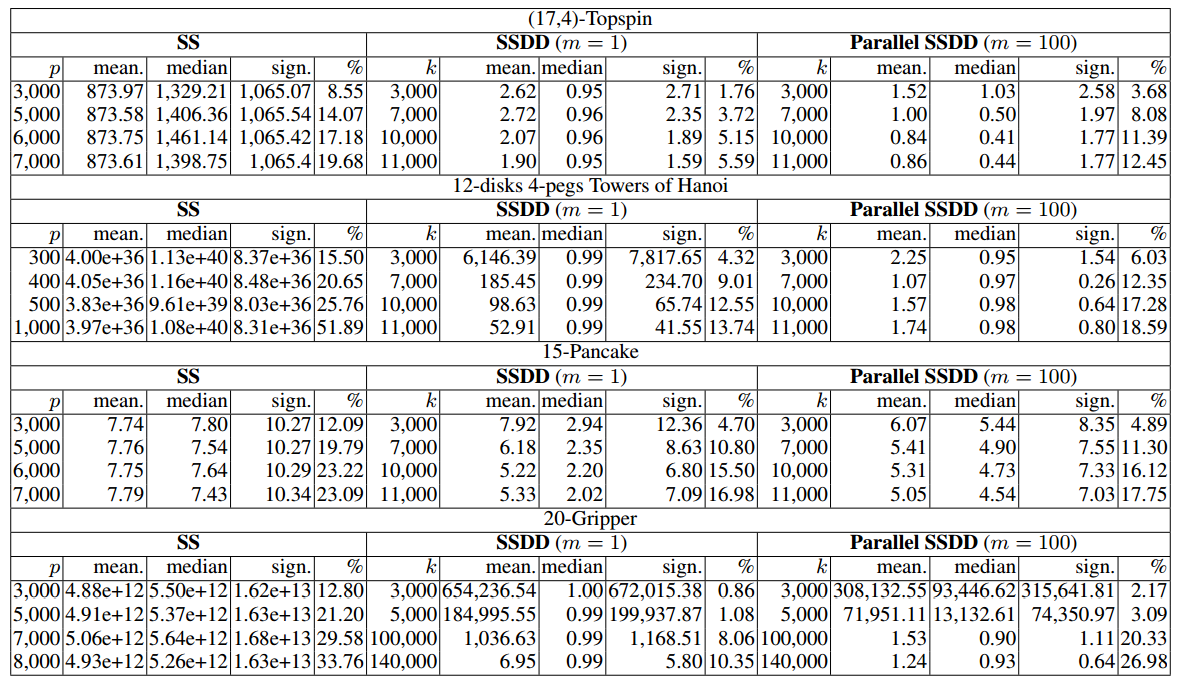
\includegraphics[scale=0.36]{lelis_fig2.png}
\end{frame}

\begin{frame}
  \frametitle{Observations and Analyses}
  \begin{itemize}
  \item SS is the worst in almost every case, increasing the number of probes doesn't help that much.
    \begin{itemize}
    \item SS doesn't account for duplicates, so it has a systematic bias toward overprediction.
    \end{itemize}
  \item SSDD is run with only 1 probe, but does much better than SS
    \begin{itemize}
    \item For each representative expanded, they run thousands of SDD walks.
    \item By not expanding duplicates, SSDD mitigates SS's bias toward overprediction.
    \end{itemize}
  \item The mean prediction for SSDD is always greater than the median
    \begin{itemize}
    \item The predictions are unevenly distributed.
    \item A small number of SSDD probes will fail to detect duplicates, and give extremely large overestimations.
    \end{itemize}
  
  \item Parallel SSDD's mean is similar to it's median.
    \begin{itemize}
    \item Parallel SSDD runs 100 probes in parallel, and stops when the first 95\% have completed.
    \item Thus cutting off the problematic 'tail' of the prediction distribution.
    \end{itemize}
    
  \end{itemize}
\end{frame}


\begin{frame}
  \frametitle{Search-radius}
  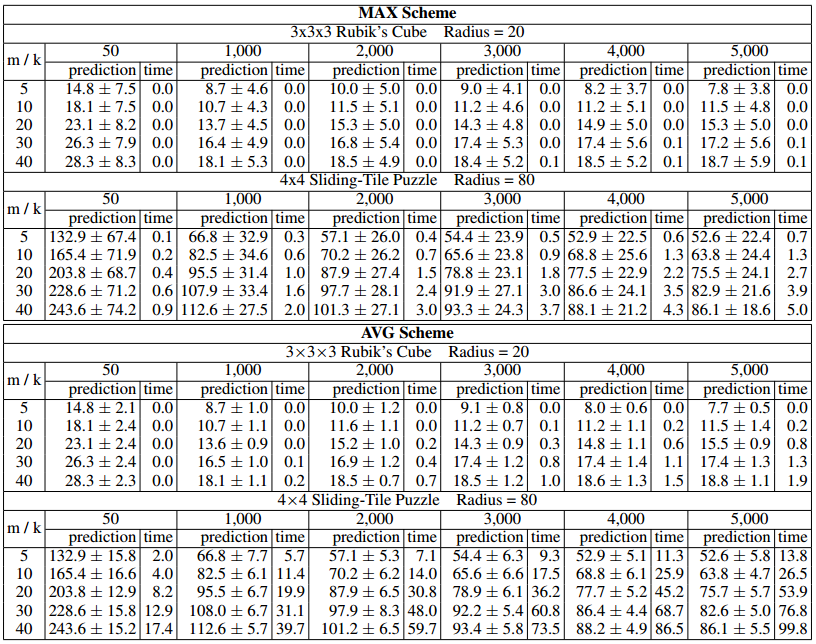
\includegraphics[scale=0.5]{lelis_fig3.png}
\end{frame}

\begin{frame}
  \frametitle{Observations and Analyses}
  \begin{itemize}
  \item Increasing the number of probes increases the predicted value
    \begin{itemize}
    \item We MAX over all probes
    \end{itemize}
  \item Increasing the number of SDD walks decreases the predicted value
    \begin{itemize}
    \item We only stop when every new representative is detected as a duplicate.
    \end{itemize}
  \item Increasing both gets us closer to the true value.
    \begin{itemize}
    \item Assuming we ran an infinite number of SDD walks so that we predicted duplicates with 100\% accuracy, then none of the probes would exceed the radius.
    \item
      If we then did an infinite number of random SSDD probes,
      eventually one of the probes will produce the actual path of the maximum optimal solution.
    \end{itemize}
  
  \item AVG reduces the variance of the predictions, but it is slower.
    \begin{itemize}
    \item AVG runs MAX a bunch of times, and then averages the results.
    \end{itemize}
    
  \end{itemize}
\end{frame}

\begin{frame}
  \frametitle{Future Research}
  \begin{itemize}
  \item There are other runtime prediction methods that could be enhanced by SSDD.
    \begin{itemize}
    \item Korf, Reid, and Edelkamp's KRE predicts IDA*.
    \item Zahavi et. al's Conditional Distribution Prediction (CDP) is an improvement of KRE.
    \end{itemize}
  \item Is there some better alternative to SDD?
    \begin{itemize}
    \item We don't want to do thousands of random walks.
    \item Move pruning is a technique that eliminates redundant sequences of operators.
    \item If we knew the probability of nodes of each type being a duplicate,
      could we use that to inform SS? (my Honours dissertation)
    \end{itemize}
  \item How can we generate a good type system automatically?
    \begin{itemize}
    \item They use \(t(n) = h(n)\) for A* and \(t(n) = |\pi(n)|\) for radius.
    \item Combine different type systems? \\
      \(t_a(n) = x\), \(t_b(n) = y\), \(t_{ab}(n) = xy\)
    \end{itemize}
  \item Can we predict the size of the reachable state space with SSDD?
    \begin{itemize}
    \item This could be used in conjunction with an abstract (PDB) search in order to estimate the size of the actual search. (find the  'Space Compression Factor')
    \end{itemize}
  \end{itemize}
\end{frame}

\begin{frame}
  \frametitle{Discussion}
  \begin{itemize}
  \item How important is the problem being addressed?
  \item How significant are the claims?
  \item How convincing is the support for these claims?
  \item How general is this approach?
  \item Does this work/approach generalise to other problems?
  \item Does this work lead on to further research?
  \end{itemize}
\end{frame}

\end{document}
